\documentclass[9pt]{beamer}

%~~~~~~~~~~~~~~~~~~~~~~~~~~~~~~~~~~~~~~~~~~~~~~~~~~~~~~~~~~~~~~~~~~~~~~~~~~~~~~
% Use roboto Font (recommended)
\usepackage[sfdefault]{roboto}
\usepackage[utf8]{inputenc}
\usepackage[french]{babel} %langue française
\usepackage[T1]{fontenc}
%~~~~~~~~~~~~~~~~~~~~~~~~~~~~~~~~~~~~~~~~~~~~~~~~~~~~~~~~~~~~~~~~~~~~~~~~~~~~~~

%~~~~~~~~~~~~~~~~~~~~~~~~~~~~~~~~~~~~~~~~~~~~~~~~~~~~~~~~~~~~~~~~~~~~~~~~~~~~~~
% Define where theme files are located. ('/styles')
\usepackage{styles/fluxmacros}
\usefolder{styles}
% Use Flux theme v0.1 beta
% Available style: asphalt, blue, red, green, gray 
\usetheme[style=asphalt]{flux}
%~~~~~~~~~~~~~~~~~~~~~~~~~~~~~~~~~~~~~~~~~~~~~~~~~~~~~~~~~~~~~~~~~~~~~~~~~~~~~~

%~~~~~~~~~~~~~~~~~~~~~~~~~~~~~~~~~~~~~~~~~~~~~~~~~~~~~~~~~~~~~~~~~~~~~~~~~~~~~~
% Extra packages for the demo:
\usepackage{booktabs}
\usepackage{colortbl}
\usepackage{ragged2e}
\usepackage{schemabloc}
%~~~~~~~~~~~~~~~~~~~~~~~~~~~~~~~~~~~~~~~~~~~~~~~~~~~~~~~~~~~~~~~~~~~~~~~~~~~~~~
%~~~~~~~~~~~~~~~~~~~~~~~~~~~~~~~~~~~~~~~~~~~~~~~~~~~~~~~~~~~~~~~~~~~~~~~~~~~~~~
% Informations
\title{Simulations Multi-Agent pour les Villes Intelligentes}
\subtitle{Une Architecture Multi-Environnement Temporelle, Spatiale et Organisationnelle. Apports pour l'Anticipation}
\author{\textbf{Présenté par : }Tahina Ralitera}
\institute{\textbf{Directeur de thèse :} Pr. Rémy Courdier\\ 
		\textbf{Co-encadrant :} Dr. Denis Payet}
\date{\today}
\titlegraphic{assets/logoUR.jpg}
%~~~~~~~~~~~~~~~~~~~~~~~~~~~~~~~~~~~~~~~~~~~~~~~~~~~~~~~~~~~~~~~~~~~~~~~~~~~~~~

\begin{document}

% Generate title page
\titlepage

% La table des matières
\begin{frame}[plain]
 \frametitle{Outline}
 \tableofcontents
\end{frame}


\section{Introduction}

\subsection{Contexte}
\begin{frame}{General Background}
\begin{columns}
\begin{column}{.48\linewidth}
\begin{block}{\visible<4->{Pressure on resources management}}
\begin{itemize}
    \visible<1->{\item Growing urbanisation}
    \visible<2->{\item Economical crises}
    \visible<3->{\item Environmental crises}
\end{itemize}
\end{block}
\end{column}
\begin{column}{.48\linewidth}
\visible<6->{
\begin{block}{\visible<6->{Contributions of ICT}}
\begin{itemize}
    \visible<7->{\item Changes in multiple level}
    \visible<8->{\item Digitalization}
    \visible<9->{\item Importance of information}
\end{itemize}
\end{block}
}
\end{column}
\end{columns}
\vspace{.3cm}
\visible<5->{
\begin{figure}
\centering
	
\includegraphics[width=.2\textwidth]{figures/question.png}
\end{figure}
}
\vspace{.3cm}
\centering \visible<10->{\alert{\huge{SMART CITY}}}
\note{
Nous faisons face à un phénomène d'urbanisation croissante accompagné de différentes crises économiques et environnementales qui engendrent d'autres crises comme la crise sanitaire que nous affrontons actuellement. Ces crises mettent une énorme pression sur la structure des villes et sur la gestion des ressources. Nous sommes alors contraints à chercher des solutions pratiques, techniques à ces différents problèmes, tout en prêtant uneattention particulière à l’environnement et au développement durable. En parallèle à cela, nous assistons, depuis ces dernières décennies à la montée en puissance des TIC qui contribue fortement à de grands changements au niveau de la ville, sur tous ses aspects : économique, culturel, transport, communication, etc. Les villes deviennent de plus en plus numériques et basées sur l’information.  Ces tendances ont conduit à la popularité du concept de ville intelligente ou smart city qui est considéré comme une solution aux problèmes évoquées précédemment.}
\end{frame}

%%%%%%%%%%%%%%%%%%%%%%%%%%%%%%%%%%%%%%%%%%%%%%%%%%%%%%%%%%%%%%%%%
\begin{frame}{General Background}{Smart City}
\begin{columns}
\begin{column}[l]{.48\linewidth}
\begin{figure}
	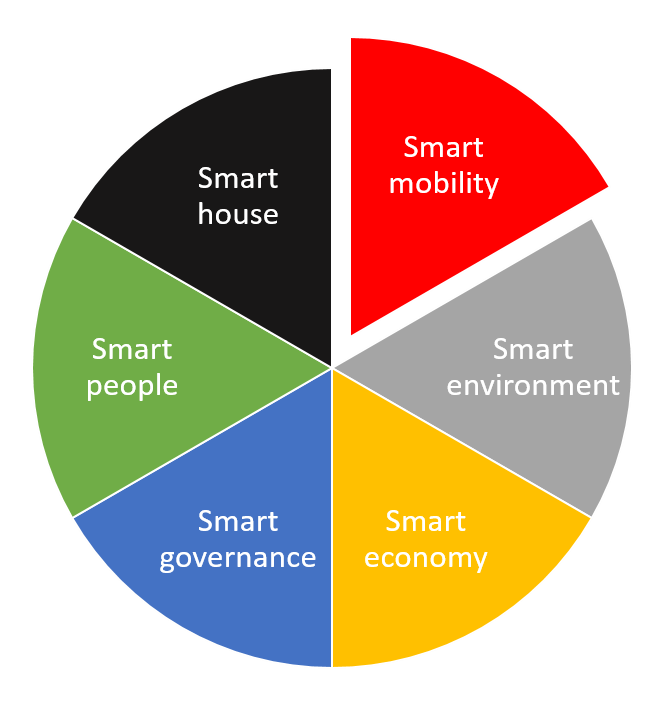
\includegraphics[width=\textwidth]{figures/smart_city.png}
\end{figure}
\end{column}
\begin{column}{.48\linewidth}
\visible<2->{\begin{block}{Criteria}
\begin{itemize}
    \item A bottom-up approach
    \item A more inclusive approach to citizens
    \item A participatory intelligence that emerges from the interactions between citizens and the system
\end{itemize}
\medbreak
\centering
\visible<3->{\alert{MULTI-AGENT SIMULATION}}
\end{block}}
\end{column}
\end{columns}
\note{\only<1>{Il n'existe pas encore de standard permettant de définir ce qu'est une ville intelligente. Plusieurs définitions peuvent se retrouver dans la littérature, mettant en valeur une ou plusieurs aspects de la ville. Celle que nous pensons la plus complète est celle de Giffinger. Giffinger défini une ville intelligente comme une ville qui est performante en 6 caractéristiques : l'environnement, l'économie, la mobilité, l'habitat, la gouvernance et le citoyen. Nous nous intéressons particulièrement à la mobilité intelligente. Cependant, nous pensons que nos solutions sont assez génériques pour être applicable aux autres domaines. Je reviendrai plus en détail sur notre cadre applicatif autour de la mobilité intelligente plus tard.}

\only<2>{Contrairement à beaucoup d'autres définitions qui ont tendance à négliger la place du citoyen ou aux mieux à les prendre en compte de façon marginale: en tant que consommateurs, dont les habitudes sont scrutées et régentées par des systèmes techniques, nous pensons que les citoyens occupent une place centrale dans la mise en oeuvre d'une ville intelligente. L'intelligence dont il est sujet ici est notamment une forme d'intelligence collective qui émerge des interactions entre le citoyen et le système. Dans ce contexte, les nouveaux outils du numérique facilitent grandement la participation des citoyens à l'élaboration des politiques, à la planification, etc. Ces citoyens échangent des informations et adoptent des comportements qui tendent à satisfaire des objectifs collectifs.}

\only<3>{L'approche multi-agent est une approche prometteuse permettant de modéliser ces types de systèmes. C'est une approche ascendante. Elle fait l'objet depuis longue date de recherches en intelligence artificielle distribuée. Appliqués au système de la ville, les sma permettent de décomposer cette dernière en plusieurs sous-ensembles plus simples, gérés par plusieurs entités autonomes, sociales, réactives et pro-actives appelées agents. Les sma permettent également de modéliser la non-linéarité et favorisent l’émergence des normes et des protocoles nécessaires pour les villes intelligentes.
\medbreak
Le domaine des sma mobilise des scientifiques issus majoritairement de l’informatique, des sciences cognitives et des systèmes complexes. Il produit un large spectre de solutions dans des champs d'applications tels que le développement de systèmes informatiques décentralisés, la résolution collective de problème, le développement de systèmes médiatisés ou encore la simulation de phénomènes complexes. C'est ce dernier champ d'application qui nous intéresse dans le cadre de nos travaux. Nous nous focalisons particulièrement sur les modèles de simulation multi-agent. Ces modèles de simulation servent à analyser le fonctionnement de scénario choisi, afin de déduire des enseignements pratiques de gestion opérationnelle dans le cadre de la conception et de la planification de villes intelligentes.}
}
\end{frame}

%%%%%%%%%%%%%%%%%%%%%%%%%%%%%%%%%%%%%%%%%%%%%%%%%%%%%%%%%%%%%%%%

\begin{frame}{Application Context}
\begin{itemize}
    \item Collective Adaptative System working group
    \item Multi-agent System :
    \begin{itemize}
        \item Focus on multi-agent simulation
        \item Hybrid approaches
    \end{itemize}
\end{itemize}


\note{
Cette thèse s’inscrit dans la continuité des travaux étudiés précédemment par le groupe de travail SCA du LIM. Notre équipe de recherche est spécialisée dans le paradigme des SMA, avec un accent particulier sur les aspects de simulations. Néanmoins, la politique actuelle de l’équipe s’oriente plus vers les approches de type hybrides. Cela veut dire qu’elle ne s’intéresse plus uniquement à la simulation, mais aussi à l’application dans un environnement réel. 
}
\end{frame}
%%%%%%%%%%%%%%%%%%%%%%%%%%%%%%%%%%%%%%%%%%
\begin{frame}{Application Context}
\begin{columns}
\begin{column}{.10\linewidth}
\begin{figure}
	
\includegraphics[width=\textwidth]{assets/icl.png}
\end{figure}
\begin{figure}
	
\includegraphics[width=\textwidth]{assets/saintDenis.png}
\end{figure}
\end{column}
\begin{column}[l]{.68\linewidth}
\begin{itemize}
    \item Multi-agent simulation of smart city and smart island : Smart mobility
    \item Multi-agent simulation of electric vehicle travel flows:
    \begin{itemize}
        \item SkuadCityModel
        \item SmartCityModel
    \end{itemize}
\end{itemize}
\vspace{1cm}
\textbf{Problem : } management of shared resources, limited in space and time
\end{column}
\end{columns}
\note{
Un des sous-thèmes développés consiste en l’application des simulations multi-agent dans le domaine des villes intelligentes et des îles intelligentes. Il s’agit d’un domaine en émergence dans notre équipe et sur lequel nous travaillons en collaboration avec des chercheurs de l'ICL et avec la mairie de Saint-Denis, La Réunion. Les problématiques abordées sont en lien avec la mobilité intelligente. Nous appliquons notre approche sur un modèle de simulation multi-agent de flux de déplacement de véhicules électriques sur un territoire que nous développons au sein même de notre équipe. Ce modèle s’appelle SkuadCityModel. Il se base sur un modèle développé par les chercheurs de l’ICL appelé SmartCityModel, sur lequel nous avons également contribué et qui a fait l'objet de deux contributions. Les problématiques abordées dans le cadre de cette thèse découlent des limites détectées lors de ces expérimentations. Nous nous intéressons notamment à des problématiques liées à la gestion de ressources partagées et limitées dans l’espace et dans le temps. Cette dernière fait partie des problèmes à l’origine même de la création du concept de ville intelligente. L’exemple sur lequel nous nous basons est celui du rechargement des véhicules électriques avec des bornes de recharge publiques.}
    
\end{frame}


%%%%%%%%%%%%%%%%%%%%%%%%%%%%%%%%%%%%%%%%%%
\begin{frame}{Application Context}{The example of the electric vehicle flow simulation}
\begin{columns}
\begin{column}{.48\linewidth}
\begin{figure}
	
\includegraphics[width=.7\textwidth]{figures/driver.png}
\end{figure}
\centering {\Large Driver}
\end{column}
\begin{column}{.48\linewidth}
\begin{figure}
	
\includegraphics[width=.7\textwidth]{figures/electric-charge.png}
\end{figure}
\centering {\Large Charging point}
\end{column}
\end{columns}
\note{La recharge de véhicules électriques implique principalement deux entités : le conducteur de voiture électrique et la borne de recharge. Ces deux entités sont autonomes et indépendantes.}
\end{frame}


%%%%%%%%%%%%%%%%%%%%%%%%%%%%%%%%%%%%%%%%%%%%%%%%%%%%%%%%%%%%%%%%%%%%%%%%%%%%%%%
\begin{frame}{Application Context}{The example of the electric vehicle flow simulation}
\alt<1-6>{
\begin{block}{Driver}
\begin{columns}
\begin{column}{.18\linewidth}
\begin{figure}
	
\includegraphics[width=\textwidth]{figures/driver.png}
\end{figure}
\end{column}
\begin{column}{.78\linewidth}
\begin{itemize}
    \visible<2->{\item Own a schedule composed of daily life activities that require travel}
    \visible<3->{\item The activities are situated in time and space}
    \visible<4->{\item \textbf{Main objective}: to accomplish all his planned activities}
    \visible<5->{\item \textbf{Main constraint}: recharging}
    \visible<6->{\item \textbf{Main strategy}: optimizing recharging
    \begin{itemize}
        \item Choosing the right time
        \item Minimise the recharging duration
    \end{itemize}
    
    }
\end{itemize}
\end{column}
\end{columns}
\end{block}
}{
\begin{block}{Charging point}
\begin{columns}
\begin{column}{.18\linewidth}
\begin{figure}
	
\includegraphics[width=\textwidth]{figures/electric-charge.png}
\end{figure}
\end{column}
\begin{column}{.78\linewidth}
\begin{itemize}
    \visible<7->{\item Limited number}
    \visible<8->{\item The availability is not guaranteed at any time or place}
    \visible<9->{\item \textbf{Main objective}: optimize its occupancy rate}
    \visible<10->{\item \textbf{Main constraint}: queue length}
    \visible<11->{\item \textbf{Main strategy}: optimize the distribution of electric vehicle recharging in its queue}
\end{itemize}
\end{column}
\end{columns}
\end{block}
}

\note{
\alt<1-6>{Dans SkuadCityModel, comme dans la réalité, un automobiliste possède un planning d'activité plus ou moins défini à l'avance. Ce planning se compose de différentes activités de la vie quotidienne nécessitant des déplacements : aller travailler, aller se divertir, rentrer chez soi ou faire ses courses. Ces activités sont situées dans le temps et dans l'espace. Cela revient à dire qu'à chaque activité, nous pouvons associer une composante spatiale (le conducteur va travailler à un endroit précis), et une composante temporelle (le conducteur part travailler à une heure précise).
\medbreak
L'objectif principal de l'automobiliste est d'accomplir l'ensemble des activités qu'il a prévues dans son planning. Pour ce faire, il se déplace en utilisant son véhicule électrique. Cependant, ce dernier possède une autonomie de batterie limitée. Par conséquent, le rechargement devient une contrainte. Le conducteur optimise alors au maximum le rechargement, de manière à ce qu'il puisse respecter son planning. Cette optimisation consiste à choisir le bon moment pour se recharger et à minimiser la durée du rechargement. Cette durée de rechargement inclut la durée d'attente au niveau de la borne de recharge.}
{
Le nombre de bornes de recharge est limité. En France par exemple, le ratio de véhicules par point de charge est de 5,7. Ce nombre peut varier en fonction de la situation géographique de la borne. Par conséquent, la disponibilité d'une borne n'est garantie ni à tout moment ni à tout endroit, car d'autres véhicules peuvent l'utiliser. Son objectif principal est d'optimiser son taux d'occupation. 
Cette situation a des répercussions tant au niveau de la borne qu'au niveau de l'automobiliste. Pour la borne, une forte demande de rechargement augmente le nombre de véhicules en attente (la longueur de la file d'attente). Elle est donc contrainte à trouver un moyen de bien gérer la répartition du rechargement des véhicules dans sa file d'attente. }
}
\end{frame}

\begin{frame}{Application Context}{The example of the electric vehicle flow simulation}
\textbf{Problem}: Management of a shared and limited resource in space and time.
\begin{itemize}
    \item lack of information for more precise reasoning.
    \item the charging point is not aware of the state of each vehicle or the schedule of the driver.
    \item no support is provided so that the driver can access all the information held by the charging point.
\end{itemize}

\note{ Ceci illustre donc un problème de gestion de ressources partagée et limitée dans l'espace et dans le temps.
\par La borne est contrainte à trouver un moyen de bien gérer la répartition du rechargement des véhicules dans sa file d'attente. Cependant, il s'agit d'une tâche difficile, car elle n'a connaissance ni de l'état de chaque véhicule ni du planning de l'automobiliste qui le conduit. Elle ne connaît donc pas la disponibilité de leur conducteur. Du côté de l'automobiliste, l'occupation des bornes et l'augmentation de la longueur de la file d'attente multiplient le temps nécessaire pour effectuer le rechargement. Elle réduit également le nombre de créneaux de rechargement disponibles. Cela constitue une contrainte qui pourrait perturber son planning et l'empêcher d'atteindre son objectif. L'automobiliste devra donc prendre en compte les informations concernant le planning et l'état de la borne dans ses décisions. Cependant, tout comme pour la borne, aucun support n'est prévu pour que l'automobiliste puisse accéder à la totalité des informations qui sont détenues par la borne.}
    
\end{frame}
\subsection{Problématiques}
\begin{frame}{Problems}
\begin{block}{Management of a shared and limited resource in space and time}
\begin{itemize}

\item The need for \alert{interaction support} to exchange spatial, social and temporal information

\item The need for \alert{reasoning} that takes into account the spatial dimension, the temporal dimension and the social dimension

\end{itemize}
\end{block}

\note{Cet exemple fait alors ressortir deux besoins sur lesquels nous apportons notre contribution :
\begin{itemize}
    \item Le besoin en support interaction spatial, social, et temporel
    \item Le besoin en raisonnement qui prenne en compte les informations partagées par le biais du support interaction. Ces informations concernent les trois (3) dimensions : spatiale, temporelle et sociale .
\end{itemize}}
\end{frame}

\begin{frame}{Contributions}
Our contributions deal with the 2 dimensions of time:
\begin{itemize}
    \item \textbf{The time representation}: topology, structure as well as the approaches that allow to model it;
    \item \textbf{The temporal reasoning}: manipulation of these representations in order to make calculations, to conduct reasoning based on them. \textbf{Anticipation}
\end{itemize}	
    
\note{Pour répondre à ces deux besoins, nous nous concentrons particulièrement sur la dimension temporelle dans les SMA. Nos contributions portent sur deux aspects de cette dimension temporelle : la représentation du temps et le raisonnement temporel. 
\par La représentation du temps peut être implicite ou explicite et traite de sa topologie, de sa structure ainsi que des approches qui permettent de le modéliser. 
Le raisonnement temporel quant à lui est lié à la manipulation de ces représentations afin d'effectuer  des calculs, conduire des raisonnements à partir de celles-ci. En intelligence artificielle, le raisonnement temporel équivaut à un raisonnement sur ce qui change au cours du temps. Cela correspond au raisonnement sur le temps. Cependant, il convient également de souligner l'existence dans des domaines spécifiques et spécialisés (systèmes temps réel, parallélisme, etc.) d'un raisonnement dans le temps qui s'intéresse au temps nécessaire pour le calcul. Cela ne nous intéresse pas puisque le temps de calcul n'est pas la préoccupation primordiale des systèmes sur lesquels nous nous penchons. Différents problèmes très souvent issus du milieu industriel sont associés au raisonnement temporel : la planification, l'ordonnancement de tâches, le suivi de processus, le diagnostic, la prédiction. Dans notre contexte, nous choisissons de nous focaliser sur l'anticipation.

Avant d’entrer plus en détails dans ces contributions, pour une meilleure compréhension, je vais expliquer brièvement comment le temps est pris en compte actuellement dans les SMA
}
\end{frame}

\begin{frame}{Taking time into account in multi-agent simulation}
\visible<1->{
\begin{block}{Multi-agent simulation model}
\visible<2->{Schematic representation of reality with a view to studying and understanding it}
\begin{itemize}
    \visible<3->{\item A set of agents}
    \begin{itemize}
        \visible<11->{\item Behavioural cycle: perception, deliberation, action/influence}
    \end{itemize}
    \visible<4->{\item An environment}
    \begin{itemize}
        \visible<7->{\item spatial and/or social}
        \visible<8->{\item contain spatial and social activation contexts data}
    \end{itemize}
    \visible<5->{\item A set of objects}
    \visible<6->{\item A set of relation}
        \begin{itemize}
        \visible<9->{\item Agents act or exert an influence on their environment}
        \visible<10->{\item Agents perceive their environment}
    \end{itemize}
\end{itemize}
\end{block}
}
\visible<1->{
\begin{block}{Simulation platform}
\end{block}
}

\note{Une simulation multi-agents peut se diviser en deux grandes parties: la plateforme de simulation ou simulateur, le modèle de simulation. Le modèles de simulation proposent une représentation schématique de la réalité en vue de l’étudier, de la comprendre. Un modèle simulation multi-agent est  composé d’un ensemble d’entités autonomes, que l’on appelle agents, situés dans un certain environnement et interagissant selon certaines relations. D’une manière plus formelle Ferber caractérise un système multi-agent par un environnement (E), un ensemble d’objets (O) situés dans E. Ces objets peuvent être perçus, créés, détruits et modifiés par les, un ensemble d’agents (A), qui sont des objets particuliers, lesquels représentent les entités actives du système, un ensemble de relations (R) qui unissent des objets (et donc des agents) entre eux.
\par Dans la plupart des modèles, l’environnement est soit un environnement spatial, soit un environnement de communication dont un cas particulier est l’environnement social. Ces environnements contiennent les données relatives aux contextes d’activation spatiales et sociales de l’agent. La relation entre l’agent et son environnement se traduit par le fait que l’agent agit ou exerce une influence sur son environnement et le perçoit. 
\par Le cycle comportemental classique d’un agent se résume alors en trois phases: une phase de perception où il récolte des informations contenues au niveau de l’environnement, une phase de délibération où l’agent active son processus de raisonnement et choisi un comportement à exécuter en fonction des percepts qu’il aura récolté et de son état interne et une phase d'action ou d’influence où l’agent agit ou essaie d’agir sur son environnement.
}
\end{frame}

\begin{frame}{Taking time into account in multi-agent simulation}
\begin{block}{Multi-agent simulation model}
\end{block}
\begin{block}{Simulation platform}
\begin{itemize}
    \item Dedicated to the multi-agent simulation model development
    \item Contain the \alert{scheduler}
    \begin{itemize}
        \item Time management : simulation activation cycle
        \item Simulated time (virtual watch) $\ne$ real time (real watch)
    \end{itemize}
    \item \textbf{Main limit }: no access to information about the temporal activation dynamics hold by the scheduler
\end{itemize}
\end{block}

\note{
La plateforme de simulation multi-agents est dédiée au développement de systèmes et simulations multi-agent. Elle peut contenir un ensemble de librairie facilitant le développement d'un modèle de simulation. Plus particulièrement, puisque nous nous intéressons au temps, les plateforme de simulations comme celles que nous utilisons dans le cadre de cette thèse contiennent une entité appelée ordonnanceur. Cet ordonnanceur est responsable de la gestion du temps en terme de cycle d’activation de la simulation. Son fonctionnement consiste en une mécanique qui fait écouler le temps, qui active les agents et met à jour les environnements en fonction d’une horloge virtuelle . Nous parlons notamment de temps simulé qui est différent du temps réel qui est notre temps astronomique. Le temps simulé est le reflet de notre temps, c'est le temps qui est mesuré par une horloge virtuelle intégrée dans le simulateur. Ce temps simulé est géré par l'ordonnanceur. Pour cela, l’ordonnanceur utilise différents approches d’ordonnancement : à pas de temps constant, événementielle, hybride, etc. La manière dont le temps est géré est différent selon l’approche utilisé, ainsi chaque approche peut avoir ses avantages et ses limites. Cependant celle que nous retiendrons est le fait que l'agent n'a pas accès aux informations sur la dynamique d'activation temporelle contenues au niveau de l'ordonnanceur de la simulation.
}
\end{frame}

\begin{frame}{Taking time into account in multi-agent simulation}
\begin{itemize}
    \item Relation between agent and scheduler
        \begin{itemize}
            \item direct link
            \item no exchange of information about the temporal activation dynamic : it is possible to share information however it is not possible to access to it.
    \end{itemize}
    \item The agent cannot take time information into account in his reasoning
    \item Accessing or perceiving contextual data and extracting relevant information from it is always the key to advancing the effectiveness of smart city functionalities.
    \item Requirements :
    \begin{itemize}
        \item medium for information exchange
        \item taking into account the temporal dimension in the agent's reasoning
    \end{itemize}
\end{itemize}




\note{
En effet La relation entre l’agent et l’ordonnanceur se fait par lien direct. En fonction de l'approche d'ordonnancement utilisé, l'agent ou le modèle de simulation détermine le rythme d’activation et le communique à l'ordonnanceur de la simulation, au niveau de la plateforme de simulation. L’ordonnanceur active donc les agents en fonction de ces informations. Nous constatons alors qu’aucun échange d’informations ne peut être effectué au niveau de la dimension temporelle. Par exemple, il n’est pas possible pour un agent d'avoir la visibilité concernant le cycle d’activation d’un autre agent. En effet, le traitement de l’information se fait dans un seul sens : en fonction de l’approche d’ordonnancement utilisé, l’agent peut avoir la possibilité de partager des informations sur son contexte d’activation et sa dynamique d’activation temporelle. Cependant, aucun support n’est prévu pour la consultation de ces données. Il peut donc y avoir partage d'information mais pas échange. Car échange signifie partage et accès. Par conséquent, il est également impossible pour l’agent de prendre en compte dans son raisonnement des informations auxquelles il n’a pas accès : c’est-à-dire des informations sur le contexte d'activation temporel. Pourtant, selon Nigonet al. , les différentes caractéristiques des villes intelligentes partagent un trait commun : elles dépendent toutes du contexte. L’accès ou la perception de données contextuelles et l’extraction d’informations pertinentes à partir de celles-ci sont toujours la clé pour faire progresser l’efficacité des fonctionnalités des villes intelligentes. 

\par Nous constatons alors un réel besoin de support permettant non seulement le partage mais également l’accès au contexte et à la dynamique d’activation temporelle, comme c’est déjà le cas pour le contexte spatial et le contexte social. Ce support doit permettre aux agents d’avoir une visibilité sur la dimension temporelle pour prendre en compte les informations du contexte d’activation temporel dans son processus de raisonnement.pre Voyons plus en détails comment nos propositions permettent de nous affranchir de ces limites.}
\end{frame}

\subsection{Contributions}
\input{slides/contribution}

\begin{frame}{Flux}{introduction}
	\justifying
 Flux is a modern style beamer presentation. It is provided as a work in progress version and may suffer from inconsistencies. Sources and complementary information are available at\\[0.3cm]
 	\centering\textbf{github.com/pvanberg/flux-beamer}
\end{frame}

\def\beamer@mytheme@style{green}
\begin{frame}[fragile]{Flux}{colors}
	\centering
	Flux provides five differents color palettes.\\
	\verb+\usetheme[style=asphalt]{flux}+\\[0.8cm]
	\newcommand{\colorRow}[1]{
	\begin{tabular}{p{4cm}cccc}
	#1 & \cellcolor{primary}\hspace*{1cm} &\cellcolor{primaryLight}\hspace*{1cm}&\cellcolor{secondary}\hspace*{1cm}&\cellcolor{tertiary}\hspace*{1cm}\\
 	\end{tabular}
 	}
 	\colorRow{Asphalt}\\[0.3cm]
	\definecolor{primaryLight}{HTML}{3a99d9}
	\definecolor{primary}{HTML}{2e81b7}
	\definecolor{secondary}{HTML}{2e81b7}
	\definecolor{tertiary}{HTML}{e76d55}
 	\colorRow{Blue}\\[0.3cm]
    \definecolor{primaryLight}{HTML}{77933c}
    \definecolor{primary}{HTML}{4f622a}
    \definecolor{secondary}{HTML}{884F4D}
    \definecolor{tertiary}{HTML}{2B3234}
 	\colorRow{Green}\\[0.3cm]
 	\definecolor{primaryLight}{HTML}{C0392B}
    \definecolor{primary}{HTML}{96281B}
    \definecolor{secondary}{HTML}{347986}
    \definecolor{tertiary}{HTML}{56423e}
 	\colorRow{Red}\\[0.3cm]
 	\definecolor{primaryLight}{HTML}{616161}
	\definecolor{primary}{HTML}{424242}
	\definecolor{secondary}{HTML}{518071}
	\definecolor{tertiary}{HTML}{8b7687}
 	\colorRow{Gray}\\[0.3cm]
\end{frame}

\subsection{fonts}

\begin{frame}[fragile]{Flux}{fonts}
 Flux recommends the use of Roboto or Overpass font and a font size of 9pt.\\[0.2cm]
 \begin{center}
 	\verb+\documentclass[9pt]{beamer}+\\
	\verb+\usepackage[sfdefault]{roboto}+
 \end{center}
 
  Flux also implements default typographies.

	\begin{itemize}
		\item Regular
		\item \alert{Alert}
		\item \example{Example}
		\item \textit{Italic}
		\item \textbf{Bold}
	\end{itemize}
	
\end{frame}

\subsection{footnotes}

\begin{frame}{Flux}{footnotes}
		Flux also includes custom footnote integration. For instance, this \textbf{element}\footnote{Footnotes are notes placed at the bottom of a page. They cite references or comment on a designated part of the text above it. For example, say you want to add an interesting comment to a sentence you have written, but the comment is not directly related to the argument of your paragraph. } and this \textbf{element}\footnote{Footnotes are not just for interesting comments, however. Sometimes they simply refer to relevant sources -- they let your reader know where certain material came from, or where they can look for other sources on the subject.} provide a footnote.
\end{frame}

\section{Collections}
\subsection{lists}

\begin{frame}{Flux}{lists}
   \begin{columns}[T,onlytextwidth]
    \column{0.33\textwidth}
      \textbf{Items}
      \begin{itemize}
        \item Cats \item Dogs \item Birds
      \end{itemize}

    \column{0.33\textwidth}
      \textbf{Enumerations}
      \begin{enumerate}
        \item First \item Second \item Last
      \end{enumerate}

    \column{0.33\textwidth}
      \textbf{Descriptions}
      \begin{description}
        \item[Apples] Yes \item[Oranges] No \item[Grappes] No
      \end{description}
\end{columns}
\let\thefootnote\relax\footnote{Note the following demo slides are directly taken from metropolis theme. Copyright 2014 Matthias Vogelgesang.\\
Give a look at https://github.com/matze/mtheme/tree/master/demo}
\end{frame}

\subsection{tables}

\begin{frame}{Flux}{tables}
  \begin{table}
    \caption{Largest cities in the world (source: Wikipedia)}
    \begin{tabular}{@{} lr @{}}
      \toprule
      City & Population\\
      \midrule
      Mexico City & 20,116,842\\
      Shanghai & 19,210,000\\
      Peking & 15,796,450\\
      Istanbul & 14,160,467\\
      \bottomrule
    \end{tabular}
    \hspace*{1cm}
        \setlength\extrarowheight{3pt}
    \begin{tabular}{|lr|}
      \hline
      \rowcolor{primaryLight}\color{background}City & \color{background}Population\\
      \hline
      Mexico City & 20,116,842\\
      Shanghai & 19,210,000\\
      Peking & 15,796,450\\
      Istanbul & 14,160,467\\
      \hline
    \end{tabular}
\end{table}
\end{frame}

\subsection{blocs}

\begin{frame}[fragile]{Flux}{blocks}
  		Flux theme comes with three pre-defined block style collections.\\
  		Native style (default) available as \verb+\setblockstyle{native}+\\[0.5cm]
  
   \setblockstyle{native} % Default behavior, optional line.
   \centering
	\begin{minipage}[b]{0.5\textwidth}

	  \begin{block}{Default}
        Block content.
      \end{block}

      \begin{alertblock}{Alert}
        Block content.
      \end{alertblock}

      \begin{exampleblock}{Example}
        Block content.
      \end{exampleblock}      
      
	\end{minipage}
	
\end{frame}

\begin{frame}[fragile]{Flux}{blocks}
  		Flux theme comes with three pre-defined block style collections.\\
  		NoBackground style available as \verb+\setblockstyle{nobackground}+\\[0.5cm]
  
   \setblockstyle{nobackground}
   \centering
	\begin{minipage}[b]{0.5\textwidth}

	  \begin{block}{Default}
        Block content.
      \end{block}

      \begin{alertblock}{Alert}
        Block content.
      \end{alertblock}

      \begin{exampleblock}{Example}
        Block content.
      \end{exampleblock}       
      
	\end{minipage}
	
\end{frame}

\begin{frame}[fragile]{Flux}{blocks}
  		Flux theme comes with three pre-defined block style collections.\\
  		Metropolis style available as \verb+\setblockstyle{metropolis}+\\[0.5cm]
  
   \setblockstyle{metropolis}
   \centering
	\begin{minipage}[b]{0.5\textwidth}

	  \begin{block}{Default}
        Block content.
      \end{block}

      \begin{alertblock}{Alert}
        Block content.
      \end{alertblock}

      \begin{exampleblock}{Example}
        Block content.
      \end{exampleblock}      
      
	\end{minipage}
	
\end{frame}

\begin{frame}{Flux}{diagrams}
\centering
\begin{tikzpicture}
    \sbEntree{E}
    \sbComp{a}{E}
    \sbBlocL{c}{$H_2$}{a}
            \sbRelier[$\epsilon$]{a}{c}
    \sbComph{d}{c}
            \sbRelier[u]{c}{d}
    \sbBlocL{e}{$H_3$}{d}
    \sbBlocL{f}{$H_4$}{e}
    \sbSortie[5]{S1}{f}
            \sbRelier{f}{S1}
            \sbNomLien[0.8]{S1}{$S_1$}
    \sbDecaleNoeudy[-4]{f}{u}
    \sbDecaleNoeudy{e}{v}
    \sbBlocr{r1}{$R_1$}{u}
    \sbBlocr{r2}{$R_2$}{v}
    \sbBlocrL{r3}{$R_3$}{r2}
    \sbRelieryx{f-S1}{r1}
    \sbRelierxy[n1]{r1}{d}
    \sbRelieryx{e-f}{r2}
    \sbRelierxy[n2]{r3}{a}
\end{tikzpicture}\\[0.4cm]
Bloc diagram example from \textbf{texample.net}
\end{frame}

\begin{frame}{Flux}{plots}
	\begin{minipage}{0.56\textwidth}
		\begin{figure}
			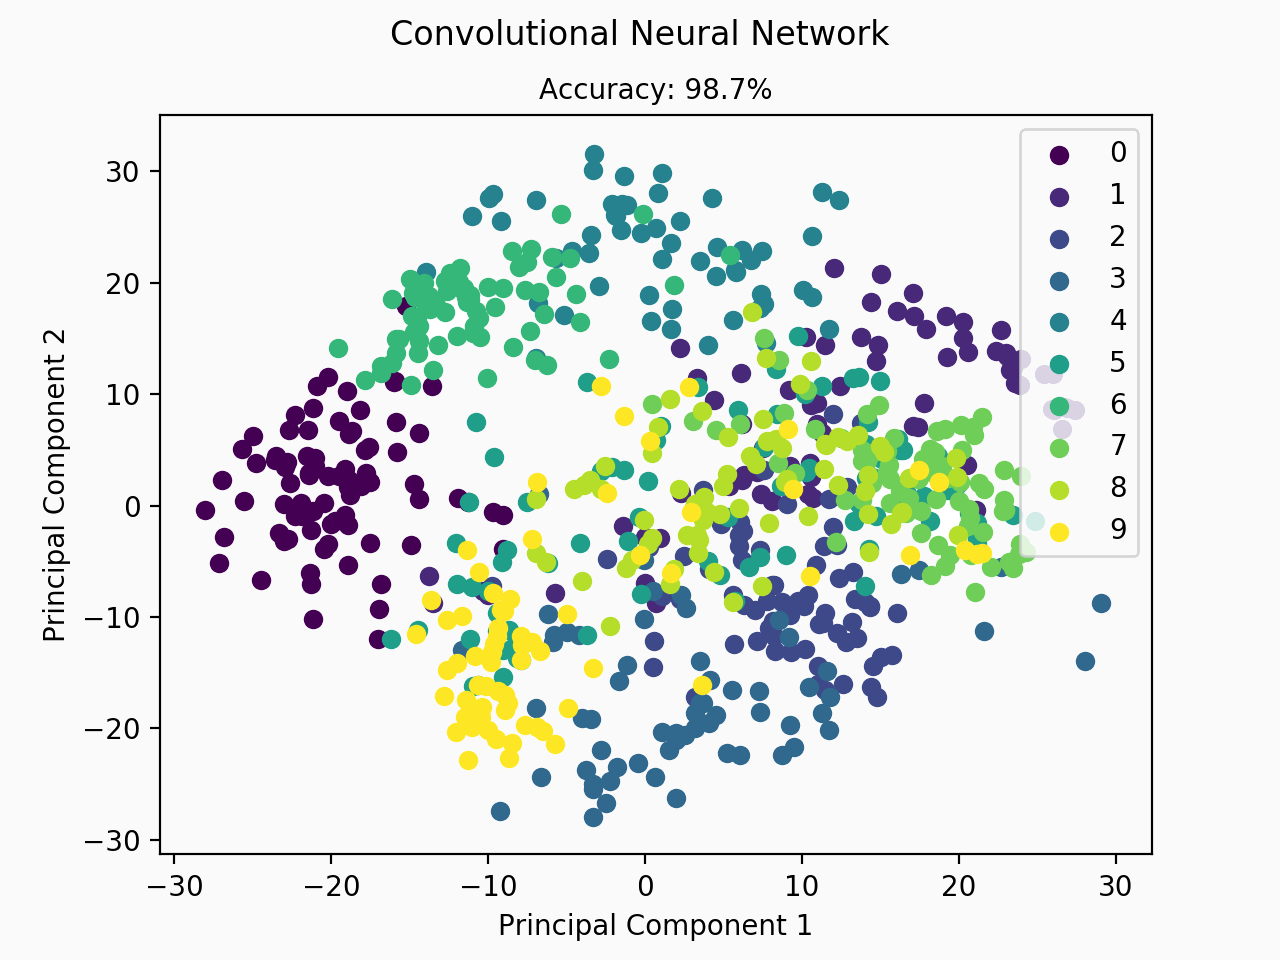
\includegraphics[width=\textwidth]{assets/plot.png}
		\end{figure}
	\end{minipage}
	\hfill
	\begin{minipage}{0.38\textwidth}
		\begin{block}{Binary Softmax classifier}
			\centering
			$\sigma(\sum_i w_ix_i + b)$
		\end{block}
		\begin{exampleblock}{Loss function}
			\centering\vspace*{0.1cm}
			$L_i = -log(\frac{e^{f_{y_i}}}{\sum_j e^{f_j}})$\\[0.1cm]
			cross entropy
		\end{exampleblock}
	\end{minipage}
\end{frame}

% The [plain] causes the headlines, footlines, and sidebars 
% to be suppressed. Useful for showing large pictures
\begin{frame}[plain]
	\begin{center}
	  This is a plain frame.\\
	  Use it to display full page images.
	  \end{center}
\end{frame}

\begin{frame}[allowframebreaks]{References}

  \nocite{*}
  \bibliography{demo}
  \bibliographystyle{abbrv}

\end{frame}

\section{Next section}
\subsection{subsection 1}
\subsection{subsection 2}
\subsection{subsection 3}
\section{One more section}
\subsection{subsection 1}
\subsection{subsection 2}
\subsection{subsection 3}

\begin{frame}
 \centering
 \frametitle{Flux}
 \framesubtitle{license}
 Flux is licensed under GNU General Public License v3.\\[0.3cm]
 	\centering\textbf{http://www.gnu.org/licenses}\\[0.3cm]
Inspired by \textbf{Metropolis} theme from Matthias Vogelgesang.\\
https://github.com/matze/mtheme 
 
\end{frame}

\end{document}